\setlength{\LTpre}{\baselineskip}
\setlength{\LTpost}{6pt}
\small
\renewcommand{\arraystretch}{1.1}
\setlength{\tabcolsep}{3pt}
\begin{longtable}{C{3.4cm}C{3.7cm}C{7.0cm}}
\caption{Ligantes comerciais e coocristalizados selecionados.}\label{tab:ligantes_comerciais_metodos}\\
\toprule Ligante & Estrutura bidimensional & Fonte da estrutura ou referência \\
\midrule
\endfirsthead
\multicolumn{3}{c}{\tablename~\thetable\ (continuação)}\\
\toprule Ligante & Estrutura bidimensional & Fonte da estrutura ou referência \\
\midrule
\endhead
\midrule
\multicolumn{3}{r}{Continua na próxima página}\\
\endfoot
\bottomrule
\endlastfoot
ARP-100 & 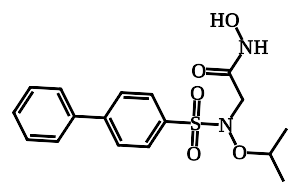
\includegraphics[width=3.2cm,height=0.9cm,keepaspectratio]{image/estruturas_ligantes_integracao/miniaturas/com_ARP_100.png} & Estrutura química consultada no PubChem \parencite{pubchem2023} \\
Ácido ascórbico & 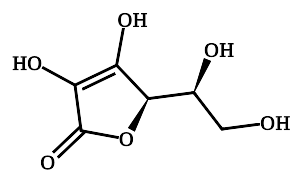
\includegraphics[width=3.2cm,height=0.9cm,keepaspectratio]{image/estruturas_ligantes_integracao/miniaturas/com_Acido_Ascorbico.png} & Estrutura química consultada no PubChem \parencite{pubchem2023} \\
Ácido kójico & 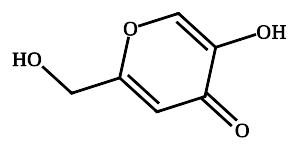
\includegraphics[width=3.2cm,height=0.9cm,keepaspectratio]{image/estruturas_ligantes_integracao/miniaturas/com_Acido_Kojico.png} & Estrutura química consultada no PubChem \parencite{pubchem2023} \\
Apigenina & 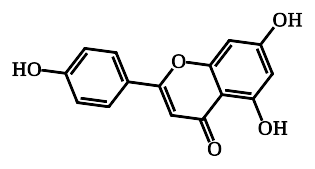
\includegraphics[width=3.2cm,height=0.9cm,keepaspectratio]{image/estruturas_ligantes_integracao/miniaturas/com_Apigenina.png} & Estrutura química consultada no PubChem \parencite{pubchem2023} \\
Arbutina & 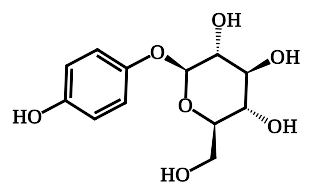
\includegraphics[width=3.2cm,height=0.9cm,keepaspectratio]{image/estruturas_ligantes_integracao/miniaturas/com_Arbutina.png} & Estrutura química consultada no PubChem \parencite{pubchem2023} \\
Batimastat & 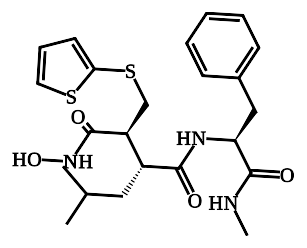
\includegraphics[width=3.2cm,height=0.9cm,keepaspectratio]{image/estruturas_ligantes_integracao/miniaturas/com_Batimastat.png} & Estrutura química consultada no PubChem \parencite{pubchem2023} \\
Cromoglicato & 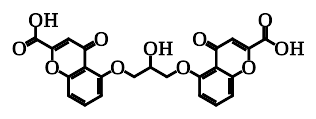
\includegraphics[width=3.2cm,height=0.9cm,keepaspectratio]{image/estruturas_ligantes_integracao/miniaturas/com_Cromoglicato.png} & Estrutura química consultada no PubChem \parencite{pubchem2023} \\
Doxiciclina & 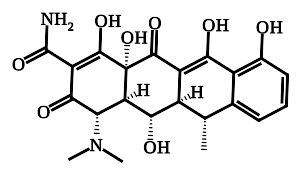
\includegraphics[width=3.2cm,height=0.9cm,keepaspectratio]{image/estruturas_ligantes_integracao/miniaturas/com_Doxiciclina.png} & Estrutura química consultada no PubChem \parencite{pubchem2023} \\
GW475151 & 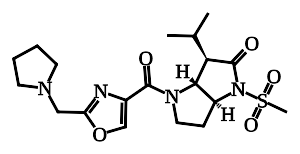
\includegraphics[width=3.2cm,height=0.9cm,keepaspectratio]{image/estruturas_ligantes_integracao/miniaturas/com_GW475151.png} & Complexo cristalográfico de elastase \parencite{macdonald2002} \\
Hidroquinona & 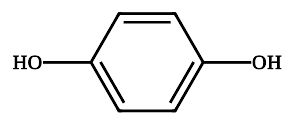
\includegraphics[width=3.2cm,height=0.9cm,keepaspectratio]{image/estruturas_ligantes_integracao/miniaturas/com_Hidroquinona.png} & Estrutura química consultada no PubChem \parencite{pubchem2023} \\
L2U & 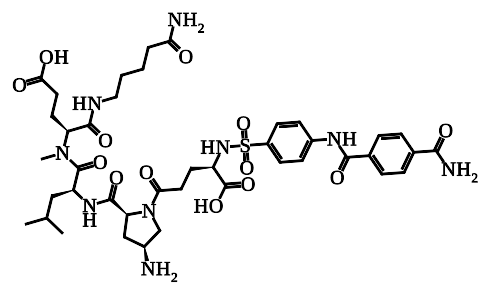
\includegraphics[width=3.2cm,height=0.9cm,keepaspectratio]{image/estruturas_ligantes_integracao/miniaturas/com_L2U.png} & Complexo cristalográfico de MMP-2 \parencite{takeuchi2023} \\
Marimastat & 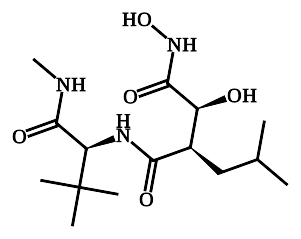
\includegraphics[width=3.2cm,height=0.9cm,keepaspectratio]{image/estruturas_ligantes_integracao/miniaturas/com_Marimastat.png} & Estrutura química consultada no PubChem \parencite{pubchem2023} \\
NFH & 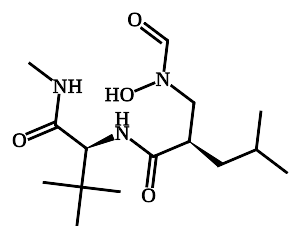
\includegraphics[width=3.2cm,height=0.9cm,keepaspectratio]{image/estruturas_ligantes_integracao/miniaturas/com_NFH.png} & Complexo cristalográfico de MMP-9 \parencite{rowsell2002} \\
PLH & 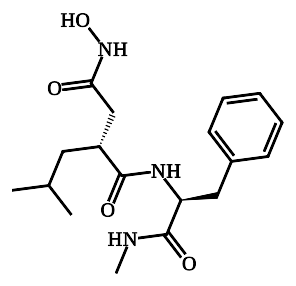
\includegraphics[width=3.2cm,height=0.9cm,keepaspectratio]{image/estruturas_ligantes_integracao/miniaturas/com_PLH.png} & Complexo cristalográfico de MMP-1 \parencite{spurlino1994} \\
Quercetina & 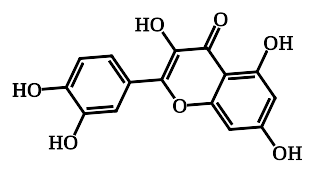
\includegraphics[width=3.2cm,height=0.9cm,keepaspectratio]{image/estruturas_ligantes_integracao/miniaturas/com_Quercetina.png} & Estrutura química consultada no PubChem \parencite{pubchem2023} \\
Sivelestat & 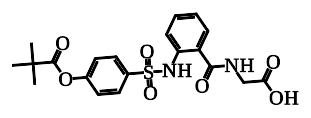
\includegraphics[width=3.2cm,height=0.9cm,keepaspectratio]{image/estruturas_ligantes_integracao/miniaturas/com_Sivelestat.png} & Estrutura química consultada no PubChem \parencite{pubchem2023} \\
Tropolona & 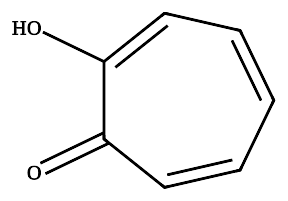
\includegraphics[width=3.2cm,height=0.9cm,keepaspectratio]{image/estruturas_ligantes_integracao/miniaturas/com_Tropolona.png} & Estrutura química consultada no PubChem \parencite{pubchem2023} \\
\end{longtable}
\normalsize
\renewcommand{\arraystretch}{1.25}
\setlength{\tabcolsep}{6pt}
